% $Header: /cvsroot/latex-beamer/latex-beamer/solutions/generic-talks/generic-ornate-15min-45min.en.tex,v 1.5 2007/01/28 20:48:23 tantau Exp $

\documentclass[aspectratio=169, bigfiles]{beamer}

% This file is a solution template for:

% - Giving a talk on some subject.
% - Style is ornate.

%\documentclass[aspectratio=169, dvipdfmx, 11pt]{beamer} % aspectratio=43, 149, 169

% Copyright 2004 by Till Tantau <tantau@users.sourceforge.net>.
%
% In principle, this file can be redistributed and/or modified under
% the terms of the GNU Public License, version 2.
%
% However, this file is supposed to be a template to be modified
% for your own needs. For this reason, if you use this file as a
% template and not specifically distribute it as part of a another
% package/program, I grant the extra permission to freely copy and
% modify this file as you see fit and even to delete this copyright
% notice.
%adapted by dw from a presentation put together by Noah Bullock.


\mode<presentation>
{
  \usetheme{Warsaw}
  % or ...Antibes, Warsaw, boxes, Boadilla,... many others

  \setbeamercovered{transparent}
  % or whatever (possibly just delete it)
}

\usepackage{here, amsmath, latexsym, amssymb, mathtools, multicol, subfig, tikz}
\usepackage{tcolorbox}
\usepackage{pgfplots}
\usetikzlibrary{patterns,matrix,arrows,arrows.meta,decorations,calc,decorations.pathreplacing,backgrounds,shapes} %arrows.metaというのを追加してしまったから悪影響があれば消す
\usetikzlibrary{decorations.pathmorphing,decorations.text}
\usetikzlibrary{scopes,decorations.markings,positioning,shapes.arrows} 
\usetikzlibrary{topaths,calc}
\usepackage{graphicx}  % Required for including images
%\usepackage{amsmath,amssymb}
\usepackage{array}
\usepackage{geometry}  %To make it easier to include mathematics
\usepackage{booktabs} % Top and bottom rules for tables
\usepackage{subfig}
\usepackage{tabularx}
\usepackage{caption}
%\usepackage[english]{babel}
% or whatever


\usepackage[latin1]{inputenc}
% or whatever

\usepackage{multicol}

\usepackage{times}
\usepackage[T1]{fontenc}
\usepackage{comment}

\usepackage{mathrsfs}  
\usepackage{hyperref}

%Graphics and Videos
%\usepackage{graphicx} %The mode "LaTeX => PDF" allows the following formats: .jpg  .png  .pdf  .mps
% \graphicspath{{./PresentationPictures/}} %Where the figures folder is located
\usepackage{media9}
% \addmediapath{./Movies/}
\usepackage{multimedia}


%%% Tomoya's imports and defs
\newcommand{\ninni}{{}^\forall} %∀
\newcommand{\aru}{{}^\exists} %∃
\newcommand{\dis}{\displaystyle} 
\newcommand{\A}{\alpha}
\newcommand{\B}{\beta}
\newcommand{\dd}{\mathrm{d}}
\newcommand{\de}{\delta}
\newcommand{\dex}{\delta_x}
\newcommand{\dey}{\delta_y}
\newcommand{\K}{\kappa}
\newcommand{\la}{\lambda}
\newcommand{\N}{\mathbb{N}}
\newcommand{\NN}{\mathcal{N}}
\newcommand{\PP}{\mathscr{P}}
\newcommand{\R}{\mathbb{R}} 
\newcommand{\RR}{\mathbb{R}_{\geq 0}}
\newcommand{\LL}{\mathcal{L}}
\newcommand{\Z}{\mathbb{Z}}
\newcommand{\ttilde}{\widetilde} %大きいチルダ
\newcommand{\eps}{\varepsilon} %ε
\newcommand{\uto}{\uparrow}
\newcommand{\dto}{\downarrow}
\newcommand{\rv}{\mathbb{R}^V} 
\newcommand{\expo}{\mathsf{exp}}
\newcommand{\vol}{\mathsf{vol}}
\newcommand{\spd}{\mathsf{spd}}
\newcommand{\mt}{\mathsf{MT}}
\newcommand{\ttt}{\mathsf{TT}}
\DeclareMathOperator\supp{supp} %supp
\newcommand{\argmax}{\mathop{\rm arg\,max}\limits} %argmax
\newcommand{\argmin}{\mathop{\rm arg\,min}\limits} %argmin
\newcommand{\rwx}{\mu_x^\alpha} %xでのr.w.
\newcommand{\rwy}{\mu_y^\alpha} %yでのr.w.
\newcommand{\wxy}{W_1\big(m_x^\alpha,m_y^\alpha\big)}
\newcommand{\whxy}{W_h\big(m_x^\alpha,m_y^\alpha\big)}
\newcommand{\kaxy}{\kappa(\alpha;x,y)}
\newcommand{\tkaxy}{\tilde{\kappa}(\alpha,h;x,y)}
\newcommand{\kxy}{\kappa(x,y)}
\newcommand{\tkxy}{\tilde{\kappa}(h;x,y)}
\newcommand{\kLLYxy}{\kappa_{\textrm{LLY}}(x,y)}
\newcommand{\lip}{\textsf{Lip}(V)}
\def\:={\coloneqq} %:=
\def\bu{$\bullet$ }
\def\comar{$\rightsquigarrow$}%ぐにゃぐにゃのヤツ
\def\dcomar{$\downrsquigarrow$}%下向きぐにゃぐにゃ
\def\kakko<#1>{\left\langle #1 \right\rangle}
\def\diam(#1){\mathsf{diam}(#1)}
%\def\vol(#1){\mathsf{vol}(#1)}
\def\W(#1){W_1\big(#1\big)}
\def\wh(#1){W_h\big(#1\big)}
\def\conv(#1){\textrm{conv}\left( #1 \right)}
\def\01{\{0,1\}}
\def\L(#1){#1\textrm{-Lip}}
\def\w-#1-Lip{\textrm{w-}$#1$\textrm{-Lip}}
\def\3|{|\hspace{-0.4mm}|\hspace{-0.4mm}|}
\def\Lip(#1){\textsf{Lip}_w^{#1}(V)}
\definecolor{hanpurple}{rgb}{0.32, 0.09, 0.98}
\def\hanpurple(#1){\textcolor{hanpurple}{#1}}
\def\red(#1){\textcolor{red}{#1}}
\definecolor{officegreen}{rgb}{0.0, 0.5, 0.0}
\def\green(#1){\textcolor{officegreen}{#1}}
%\def\officegreen(#1){\textcolor{Forestofficegreen}{#1}}

\hypersetup{
colorlinks=true,
citecolor=blue,
linkcolor=red,
urlcolor=orange}

\newtcolorbox{mybox}[1]
{
    title=#1, 
    toptitle=0mm, bottomtitle=0mm, 
    colframe=structure,boxrule=5pt,
    coltitle=white, colbacktitle=structure,
    colback=white, fonttitle=\bfseries,
    top=0mm, bottom=0mm, left=0mm, right=0mm, %内部余白調整
    enlarge top by=1mm, enlarge bottom by=5mm,  %外部余白調整
}
%%%

%%% Gabe's imports and defs

\usepackage{listings}
\usepackage{pythonhighlight}
%%%

\expandafter\def\expandafter\insertshorttitle\expandafter{%
    \insertshorttitle\hfill\insertframenumber\,/\,\inserttotalframenumber}
    
    
%%%%%%Katelynn's imports

%%%%%%%%%%%%%%%%%%%%%%%%%%%%%%%%%%%%%%%%%%%%%%%%%%%%%%%%%%%%%%%%%%%%%%%%%%%%%%
% \embedvideo{<poster or text>}{<video file (MP4+H264)>}
% \embedvideo*{...}{...}                     % auto-play
%%%%%%%%%%%%%%%%%%%%%%%%%%%%%%%%%%%%%%%%%%%%%%%%%%%%%%%%%%%%%%%%%%%%%%%%%%%%%%
\usepackage[bigfiles]{pdfbase}
\ExplSyntaxOn
\NewDocumentCommand\embedvideo{smm}{
  \group_begin:
  \leavevmode
  \tl_if_exist:cTF{file_\file_mdfive_hash:n{#3}}{
    \tl_set_eq:Nc\video{file_\file_mdfive_hash:n{#3}}
  }{
    \IfFileExists{#3}{}{\GenericError{}{File~`#3'~not~found}{}{}}
    \pbs_pdfobj:nnn{}{fstream}{{}{#3}}
    \pbs_pdfobj:nnn{}{dict}{
      /Type/Filespec/F~(#3)/UF~(#3)
      /EF~<</F~\pbs_pdflastobj:>>
    }
    \tl_set:Nx\video{\pbs_pdflastobj:}
    \tl_gset_eq:cN{file_\file_mdfive_hash:n{#3}}\video
  }
  %
  \pbs_pdfobj:nnn{}{dict}{
    /Type/RichMediaInstance/Subtype/Video
    /Asset~\video
    /Params~<</FlashVars (
      source=#3&
      skin=SkinOverAllNoFullNoCaption.swf&
      skinAutoHide=true&
      skinBackgroundColor=0x5F5F5F&
      skinBackgroundAlpha=0.75
    )>>
  }
  %
  \pbs_pdfobj:nnn{}{dict}{
    /Type/RichMediaConfiguration/Subtype/Video
    /Instances~[\pbs_pdflastobj:]
  }
  %
  \pbs_pdfobj:nnn{}{dict}{
    /Type/RichMediaContent
    /Assets~<<
      /Names~[(#3)~\video]
    >>
    /Configurations~[\pbs_pdflastobj:]
  }
  \tl_set:Nx\rmcontent{\pbs_pdflastobj:}
  %
  \pbs_pdfobj:nnn{}{dict}{
    /Activation~<<
      /Condition/\IfBooleanTF{#1}{PV}{XA}
      /Presentation~<</Style/Embedded>>
    >>
    /Deactivation~<</Condition/PI>>
  }
  %
  \hbox_set:Nn\l_tmpa_box{#2}
  \tl_set:Nx\l_box_wd_tl{\dim_use:N\box_wd:N\l_tmpa_box}
  \tl_set:Nx\l_box_ht_tl{\dim_use:N\box_ht:N\l_tmpa_box}
  \tl_set:Nx\l_box_dp_tl{\dim_use:N\box_dp:N\l_tmpa_box}
  \pbs_pdfxform:nnnnn{1}{1}{}{}{\l_tmpa_box}
  %
  \pbs_pdfannot:nnnn{\l_box_wd_tl}{\l_box_ht_tl}{\l_box_dp_tl}{
    /Subtype/RichMedia
    /BS~<</W~0/S/S>>
    /Contents~(embedded~video~file:#3)
    /NM~(rma:#3)
    /AP~<</N~\pbs_pdflastxform:>>
    /RichMediaSettings~\pbs_pdflastobj:
    /RichMediaContent~\rmcontent
  }
  \phantom{#2}
  \group_end:
}
\ExplSyntaxOff
%%%%%%%%%%%%%%%%%%%%%%%%%%%%%%%%%%%%%%%%%%%%%%%%%%%%%%%%%%%%%%%%%%%%%%%%%%%%%%






%%%%%%%%%Subcaption



 \title[Mitsubishi A]{Map-matching}

%\subtitle
%{Presentation Subtitle} % (optional)

\author[T. Akamatsu, G. Gress, K. Huneycutt, S. Omura]{T. Akamatsu, G. Gress, K. Huneycutt, S. Omura \\
Academic Mentor: Dr. Kano \\
Industry Mentor: Dr. Yamazaki}


%\institute{College of Charleston}


\date[15/07] % (optional)
{\quad July 15, 2022 \\  \quad g-RIPS}


 
 
 
\pgfplotsset{compat=1.18}
\begin{document}

% \title[Mitsubishi A]{Map-matching}

% %\subtitle
% %{Presentation Subtitle} % (optional)

% \author[T. Akamatsu, G. Gress, K. Huneycutt, S. Omura]{\quad T. Akamatsu, G. Gress, K. Huneycutt, S. Omura} 

% %Academic Mentor: S. Kano \\ Industry Mentor: M. Yamazaki
% %\institute{College of Charleston}


% \date[15/07] % (optional)
% {\quad July 15, 2022 \\  \quad g-RIPS}



%\pgfplotsset{compat=1.15}



\begin{frame}
\titlepage

%\vspace{-.5cm}
%\vspace{-3.5cm}
%\hspace{-.2cm}

\end{frame}



% \begin{frame}{Outline}
%   \tableofcontents
% %   You might wish to add the option [pausesections]
% \end{frame}


\section{Introduction to map-matching}
\begin{frame}{Map-matching}
    
Given GPS trajectory data and a road map, \textbf{map-matching} is the process of
determining the route on the map that corresponds to the trajectory data.\\ 
\begin{figure}
\centering
\begin{minipage}{.5\textwidth}
\centering
  \includegraphics[scale=.1]{googlemaps.png}
  \captionof*{figure}{Web mapping services}
  \label{fig:test1}
\end{minipage}%
\begin{minipage}{.5\textwidth}
\centering
  \includegraphics[scale=.48]{selfdriving.jpeg}
  \captionof*{figure}{Autonomous Vehicles \cite{H}}
  \label{fig:test2}
\end{minipage}
\end{figure}
\end{frame}


\begin{frame}{Problem Statement}
\begin{center}
    \embedvideo{\includegraphics[page=1]{example-movie}}{traj9.mp4}   
\end{center}
\end{frame}

% \begin{frame}{Problem Statement}
% \begin{center}
%     \embedvideo{\includegraphics[page=1]{example-movie}}{traj21.mp4}   
% \end{center}
% \end{frame}


\begin{frame}{Problem Statement}
Let us fix $d \geq 2$ (but almost everywhere we consider the case $d = 2$).
\begin{definition}[Trajectory] \label{Tr}
A \textbf{trajectory} $Tr$ is a sequence of points $\mathbf{p} = (p_1,p_2,\dots, p_n)$ where $p_i\in \R^d$ for $1\leq i\leq n$ equipped with 
\begin{itemize}
    \item a sequence $t(\mathbf{p}) = (t_1,\dots,t_{n})$ such that $t_i\in \R^{+}$ for $1\leq i\leq n$ and  $t_1<t_2<\dots <t_n$, called the \textbf{timestamp} of $\mathbf{p}$,
    \item a sequence ${\spd}(\mathbf{p}) = ({\spd}_1,\dots,{\spd}_{n})$ such that $\spd_i\in \R^{+}$ for $1\leq i\leq n$, called the \textbf{speed} of $\mathbf{p}$ (optional),
    \item a sequence $u(\mathbf{p}) = (u_1, \dots, u_n)$ such that $u_i\in \R^d$ and $\|u\|=1$ for $1\leq i\leq n$, called the \textbf{direction} of $\mathbf{p}$ (optional).
\end{itemize}
\end{definition}
\end{frame}



\begin{frame}{Problem Statement}
\begin{definition}[Road Network] \label{RN}
A  \textbf{road network} (also known as a map) is a directed graph $G=(V,E)$ consists of the set $V$ (resp. $E$) of vertices (resp. edges) with an embedding $\phi:|G|\rightarrow\mathbb{R}^{d}$ of the geometric realization $|G|$ of $G$.
% , and a map $f:E\rightarrow \{(x,y)\mid  (x,y)\in V^2 \}$ where $f = (f_1,f_2) $.
We will identify $G$ and the image $\phi(|G|)$ by $\phi$ as long as there is no confusion.
\end{definition}
\end{frame}

\begin{frame}{Problem Statement}
\begin{figure}
    \centering
    \includegraphics[scale=.405]{roadnetwork9.png}
%    \caption{Caption}
%    \label{fig:my_label}
\end{figure}

\end{frame}


\begin{frame}{Problem Statement}
\begin{definition}[Route]
A \textbf{route} $r$ on a road network $G=(V,E)$ is a sequence of connected edges $(e_1,e_2,\dots,e_n)\subset E$, i.e. 
% $e_i\in E$ and $f_2(e_i) = f_1(e_{i+1})$.
the head of $e_i$ coincides with the tail of $e_{i+1}$ for each $i = 1, 2, \dots, n-1$.
Let $R$ denote the set of all routes.
\end{definition}
\end{frame}

\begin{frame}{Problem Statement}
\begin{center}
    \embedvideo{\includegraphics[page=1]{example-movie}}{route9.mp4} \end{center}
\end{frame}

\begin{frame}{Problem Statement}
\begin{figure}
    \centering
    \includegraphics[scale =.405]{route9.png}
   % \caption{Caption}
    %\label{fig:my_label}
\end{figure}
\end{frame}


\begin{frame}{Problem Statement}

\begin{definition}[Map-Matching]
Given a road network $G=(V, E)$ and a trajectory
$Tr$, the map-matching, $\mathcal{MR}_G(Tr)$, is the route that is the argument of the minimum of some function $L:R\rightarrow \mathbb{R}^+$, called the \textbf{loss function}. 
\end{definition}

\end{frame}


\begin{frame}{Approaches to Map-Matching}
\textbf{Geometric}
\begin{itemize} 
    \item Point-to-point method
    \item Point-to-curve method
\end{itemize}
\vspace{.5cm}
\textbf{Data-Driven}
\begin{itemize} 
    \item Hidden Markov model
\end{itemize}
\end{frame}


\begin{frame}{Point-to-Curve Method}
\begin{center}
    
\begin{tikzpicture}[scale=.6] %every node/.style={circle,fill=white}

\node (p1) at  (.9,2.5) {{\small \red($p_1$)}};
\node (p2) at  (.5,1.5) {{\small \red($p_2$)}};
\node (p3) at  (1.5,-.15) {{\small \red($p_3$)}};
\node (p4) at  (4,.5) {{\small \red($p_4$)}};
\node (p5) at  (5.5,-1.5) {{\small \red($p_5$)}};
\node (p6) at  (7.5,-3) {{\small \red($p_6$)}};
\node (p7) at  (9.5,-3) {{\small \red($p_7$)}};
\draw (0,3.25) node (v1) [draw] {$v_1$ };
\draw (6,3.25) node (v2) [draw] {$v_2$ };
\draw (-6,0.25) node (v3) [draw] {$v_3$ };
\draw (0,0.25) node (v4) [draw] {$v_4$ };
\draw (6,0.25) node (v5) [draw] {$v_5$ };
\draw (12,0.25) node (v6) [draw] {$v_6$ };
\draw (-6,-3.25) node (v7) [draw] {$v_7$ };
\draw (0,-3.25) node (v8) [draw] {$v_8$ };
\draw (6,-3.25) node (v9) [draw] {$v_9$ };
\draw (12,-3.25) node (v10) [draw] {$v_{10}$};
\draw (0,-6.25) node (v11) [draw] {$v_{11}$};
\draw (6,-6.25) node (v12) [draw] {$v_{12}$};

\draw (v1)--(v2);
\draw (v1)--(v4);
\draw (v2)--(v5);
\draw (v3)--(v4);
\draw (v4)--(v5);
\draw (v5)--(v6);
\draw (v3)--(v7);
\draw (v4)--(v8);
\draw (v5)--(v9);
\draw (v6)--(v10);
\draw (v7)--(v8);
\draw (v8)--(v9);
\draw (v9)--(v10);
\draw (v8)--(v11);
\draw (v9)--(v12);
\draw (v11)--(v12);
\end{tikzpicture}

\end{center}
\end{frame}

\begin{frame}{Point-to-Curve Method}
\begin{center}
    
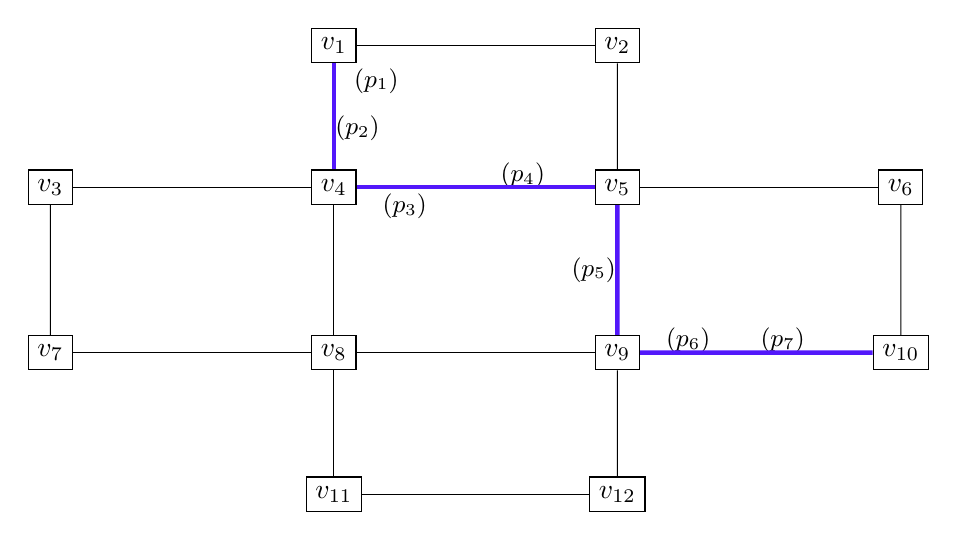
\begin{tikzpicture}[scale=.6] %every node/.style={circle,fill=white}

\node (p1) at  (.9,2.5) {{\small \red($p_1$)}};
\node (p2) at  (.5,1.5) {{\small \red($p_2$)}};
\node (p3) at  (1.5,-.15) {{\small \red($p_3$)}};
\node (p4) at  (4,.5) {{\small \red($p_4$)}};
\node (p5) at  (5.5,-1.5) {{\small \red($p_5$)}};
\node (p6) at  (7.5,-3) {{\small \red($p_6$)}};
\node (p7) at  (9.5,-3) {{\small \red($p_7$)}};
\draw (0,3.25) node (v1) [draw] {$v_1$ };
\draw (6,3.25) node (v2) [draw] {$v_2$ };
\draw (-6,0.25) node (v3) [draw] {$v_3$ };
\draw (0,0.25) node (v4) [draw] {$v_4$ };
\draw (6,0.25) node (v5) [draw] {$v_5$ };
\draw (12,0.25) node (v6) [draw] {$v_6$ };
\draw (-6,-3.25) node (v7) [draw] {$v_7$ };
\draw (0,-3.25) node (v8) [draw] {$v_8$ };
\draw (6,-3.25) node (v9) [draw] {$v_9$ };
\draw (12,-3.25) node (v10) [draw] {$v_{10}$};
\draw (0,-6.25) node (v11) [draw] {$v_{11}$};
\draw (6,-6.25) node (v12) [draw] {$v_{12}$};

\draw (v1)--(v2);
\draw[ultra thick,hanpurple] (v1)--(v4);
\draw (v2)--(v5);
\draw (v3)--(v4);
\draw[ultra thick,hanpurple] (v4)--(v5);
\draw (v5)--(v6);
\draw (v3)--(v7);
\draw (v4)--(v8);
\draw[ultra thick,hanpurple] (v5)--(v9);
\draw (v6)--(v10);
\draw (v7)--(v8);
\draw (v8)--(v9);
\draw[ultra thick,hanpurple] (v9)--(v10);
\draw (v8)--(v11);
\draw (v9)--(v12);
\draw (v11)--(v12);
\end{tikzpicture}

\end{center}
\end{frame}





% \begin{frame}{Proof of Theorem $1^*$}
% \begin{multicols}{2}
% Suppose we have a network with \textbf{bounded branching}: networks such that each vertex has no more than two edges originating from it.
% \vspace{-1.5cm}
% \small{
% \begin{align*}
%     A &= (0,0,0)  \\
%     B &= (4\sqrt{n},0,0) \\
%     C &= (4\sqrt{n},2\sqrt{n},0)\\
%     D &= (0,2\sqrt{n},0)\\
%     A' &=(0,0,8\sqrt{n}) \\
%     B' &=  (4\sqrt{n},0,8\sqrt{n})\\
%     C' &= (4\sqrt{n},2\sqrt{n},8\sqrt{n})\\
%     D' &= (0,2\sqrt{n},8\sqrt{n}))
% \end{align*}}
% \includegraphics[scale=.425]{Parallelol.png}
% \end{multicols}
% \end{frame}

\section{``Wasserstein" method}

\begin{frame}{Problem \& Our strategy}
%\vspace{-3mm}
\begin{itemize}
    \item
    A square model.
\end{itemize}
\begin{figure}[H]
\begin{center}
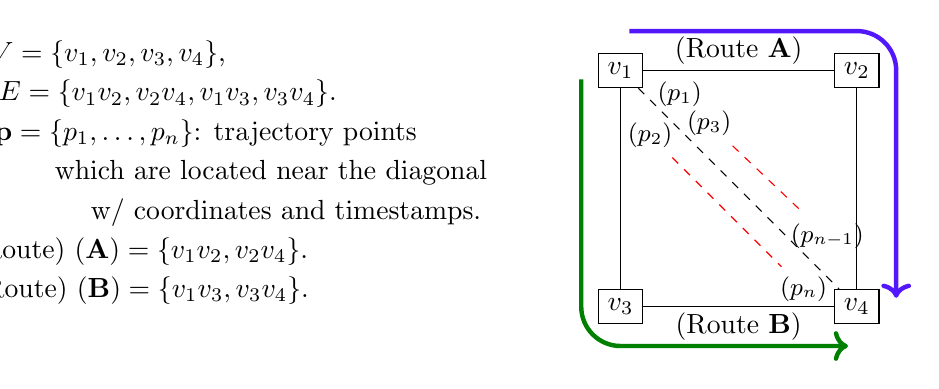
\begin{tikzpicture} %[every node/.style={circle,fill=white}] 
\node (text1) at (-4,3.2) {\hspace{-53mm}\bu $V=\{v_1,v_2,v_3,v_4\}$,};
\node (text2) at (-4,2.7) {\hspace{-35mm}$E=\{v_1v_2,v_2v_4,v_1v_3,v_3v_4\}$.};
\node (text3) at (-5,2.2) {\hspace{-8.3mm}\bu $\mathbf{p}=\{p_1,\ldots,p_n\}$: trajectory points};
\node (text4) at (-4,1.7) {\hspace{-10mm} which are located near the diagonal};
\node (text5) at (-4,1.2) {\hspace{-5mm}w/ coordinates and timestamps.};
\node (text6) at (-4,0.7) {\hspace{-45.1mm}\bu \hanpurple(Route) $\hanpurple(\mathbf{A})=\{v_1v_2,v_2v_4\}$.};
\node (text7) at (-4,0.2) {\hspace{-44.7mm}\bu \green(Route) $\green(\mathbf{B})=\{v_1v_3,v_3v_4\}$.};
\node (p1) at (0.75,2.7) {{\small \red($p_1$)}};
\node (p2) at (0.375,2.175) {{\small \red($p_2$)}};
\node (p3) at (1.125,2.325) {{\small \red($p_3$)}};
\node (pn-1) at (2.625,0.9) {{\small \red($p_{n-1}$)}};
\node (pn) at (2.325,0.225) {{\small \red($p_n$)}};
\draw (0,3) node (v1) [draw] {$v_1$};
\draw (3,3) node (v2) [draw] {$v_2$};
\draw (0,0) node (v3) [draw] {$v_3$};
\draw (3,0) node (v4) [draw] {$v_4$};
\draw (v1)--(v2);
\draw (v2)--(v4);
\draw (v4)--(v3);
\draw (v3)--(v1);
\draw[dashed] (v1)--(v4);
\draw[red, dashed] (p3)--(pn-1);
\draw[red, dashed] (p2)--(pn);
\node at (1.5,3.25) {{\hanpurple(Route $\mathbf{A}$)}};
\node at (1.5,-0.25) {{\green(Route $\mathbf{B}$)}};
\path[arrows=->, ultra thick, draw=hanpurple] ($(v1)+(0.1125,0.5)$) 
to[out=0,in=180] ($(v2)+(0,0.5)$)
to[out=0,in=90] ($(v2)+(0.5,0)$)
to[out=270,in=90] ($(v4)+(0.5,0.1125)$);
\path[arrows=->, ultra thick, draw=officegreen] ($(v1)+(-0.5,-0.1125)$) 
to[out=270,in=90] ($(v3)+(-0.5,0)$)
to[out=270,in=180] ($(v3)+(0,-0.5)$)
to[out=0,in=180] ($(v4)+(-0.1125,-0.5)$);
\end{tikzpicture}
\end{center}
\end{figure} 

\vspace{-4mm}
\begin{tcolorbox}[colframe=yellow,
colback=yellow!10!white,
colbacktitle=yellow!40!white,
coltitle=black, fonttitle=\bfseries]
\textbf{Strategy}: Construction of the ``\textbf{trajectory-to-route}"-type method.
\end{tcolorbox}
\end{frame}

\begin{frame}{``Wasserstein" method}
\vspace{-1mm}
%\begin{tcolorbox}[colframe=hanpurple,
%colback=black!10!white,
%colbacktitle=hanpurple!40!white,
%coltitle=black, fonttitle=\bfseries]
\begin{definition}[($L^1$-)Wasserstein distance \; (``\emph{$W_1$ distance}")]
%{\underline{\textbf{($L^1$-)Wasserstein distance}}}
{\small 
Let $(X,d)$ be a complete and separable metric space. \\
For $\mu,\nu\in\mathscr{P}(X)\:=\big\{\text{ all (Borel) probability measures on }(X,d)\text{ \red(w/ finite support) }\big\}$, define
$$
    W_1(\mu,\nu)\:=\min_{\pi\in\Pi(\mu,\nu)} \sum_{x\in X}\sum_{y\in X} d(x,y)\pi(x,y),
$$
where $\pi\in\Pi(\mu,\nu)$ $\;:\Leftrightarrow\;$ $\ninni x,y\in X$,\; $\sum_{y\in X}\pi(x,y)=\mu(x),\;\sum_{x\in X}\pi(x,y)=\nu(y)$. 
}
%\end{tcolorbox}
\end{definition}
\vspace{-2mm}
\begin{itemize}
    %\item {\small The right-hand side attains its minimum value.}
    \item {\small $W_1$ distance is a distance function on $\mathscr{P}(X)$, i.e. quantifies the differences between two probability measures.}
    \item {\small $W_1$ distance can be calculated by linear programming (under our setting conditions).}
    \item {\small $W_1$ distance is also called ``\textbf{Earth-Mover's distance}" or ``\textbf{Word-Mover's distance}" (in areas such as Natural Language Processing).}
\end{itemize}
\end{frame}

\begin{frame}
\vspace{-9mm}
\begin{figure}[H]
\begin{tabular}{ccc}
\begin{minipage}{0.43\hsize}
\begin{center}
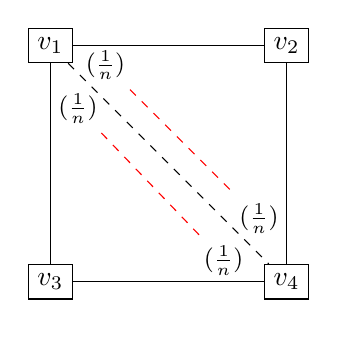
\begin{tikzpicture} %[every node/.style={circle,fill=white}]
\node (p1) at (0.7,2.75) {\small{\red($\frac{1}{n}$)}};
\node (p2) at (0.35,2.2) {\small{\red($\frac{1}{n}$)}};
\node (pn-1) at (2.65,0.8) {\small{\red($\frac{1}{n}$)}};
\node (pn) at (2.2,0.27) {\small{\red($\frac{1}{n}$)}};
\draw (0,3) node (v1) [draw] {$v_1$};
\draw (3,3) node (v2) [draw] {$v_2$};
\draw (0,0) node (v3) [draw] {$v_3$};
\draw (3,0) node (v4) [draw] {$v_4$};
\node (x) at (1.5,3) {};
\node (y) at (1.5,-0.5) {};
\draw (v1)--(v2);
\draw (v2)--(v4);
\draw (v4)--(v3);
\draw (v3)--(v1);
\draw[dashed] (v1)--(v4);
\draw[red, dashed] (p1)--(pn-1);
\draw[red, dashed] (p2)--(pn);
\end{tikzpicture}
\vspace{-4mm}
\caption{{\footnotesize A prob. meas. \red($\mu_\mathbf{p}$) associated w/ the trajectory $\mathbf{p}$. A weight $1/n$ is placed on each trajectory point; $\red(\mu_\mathbf{p})\:=(1/n)\sum_{i=1}^n \delta_{p_i}$.}}
\end{center}
\end{minipage}
%%%%%%%%%%%%%%%%%%%%%%%%%%%%%%%%%%%%%%%%%%%%%%%%%%%%%%%%%%%%%%%%%%%%%%%%%%%%%%%%%%%%%%%%%%%%%%%%%%%%%%%%%%%%%%%%%%%%%%%%%%%%%%%%%%%%%%%%%%%%%%%%%%%%%%%%%%%%%%%%%%%%%%%
\begin{minipage}{0.1\hsize}
\begin{center}
\end{center}
\end{minipage}
%%%%%%%%%%%%%%%%%%%%%%%%%%%%%%%%%%%%%%%%%%%%%%%%%%%%%%%%%%%%%%%%%%%%%%%%%%%%%%%%%%%%%%%%%%%%%%%%%%%%%%%%%%%%%%%%%%%%%%%%%%%%%%%%%%%%%%%%%%%%%%%%%%%%%%%%%%%%%%%%%%%%%%%
\begin{minipage}{0.43\hsize}
\begin{center}
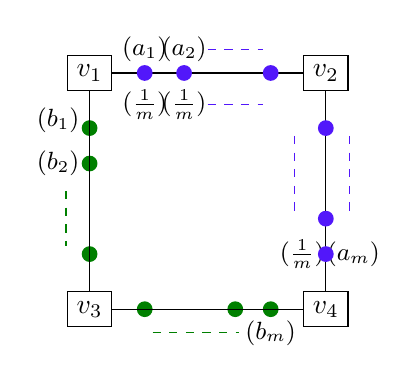
\begin{tikzpicture} %[every node/.style={circle,fill=white}]
\node (a1) at (0.7,3.3) {\small{\hanpurple($a_1$)}};
\node (p1) at (0.7,2.6) {\small{\hanpurple($\frac{1}{m}$)}};
\node (a2) at (1.2,3.3) {\small{\hanpurple($a_2$)}};
\node (p2) at (1.2,2.6) {\small{\hanpurple($\frac{1}{m}$)}};
\draw[dashed, hanpurple] (1.5,3.3)--(2.2,3.3);
\draw[dashed, hanpurple] (1.5,2.6)--(2.2,2.6);
\draw[dashed, hanpurple] (3.3,2.2)--(3.3,1.2);
\draw[dashed, hanpurple] (2.6,2.2)--(2.6,1.2);
%\node (am-1) at (3.5,1.25) {\small{\hanpurple($a_{m-1}$)}};
\node (am) at (3.35,0.7) {\small{\hanpurple($a_m$)}};
\node (pm) at (2.7,0.7) {\small{\hanpurple($\frac{1}{m}$)}};
\node (b1) at (-0.4,2.4) {\small{\green($b_1$)}};
\node (a2) at (-0.4,1.85) {\small{\green($b_2$)}};
\draw[dashed, officegreen] (-0.3,1.5)--(-0.3,0.8);
\draw[dashed, officegreen] (0.8,-0.3)--(1.9,-0.3);
%\node (am-1) at (1.8,-0.3) {\footnotesize{\officegreen($b_{m-1}$)}};
\node (am) at (2.3,-0.3) {\small{\green($b_m$)}};
\fill [officegreen] (0,2.3) circle (0.1);
\fill [officegreen] (0,1.85) circle (0.1);
\fill [officegreen] (0,0.7) circle (0.1);
\fill [officegreen] (0.7,0) circle (0.1);
\fill [officegreen] (1.85,0) circle (0.1);
\fill [officegreen] (2.3,0) circle (0.1);
%\draw[arrows=->, thick, draw=officegreen] ($(v1)+(-0.6,-0.15)$) to ($(v3)+(-0.6,-0.3)$);
%\draw[arrows=->, thick, draw=officegreen] ($(v3)+(-0.6,-0.6)$) to ($(v4)+(0,-0.6)$);
%\node at (-1.5,2) {{Route $B$}};
\draw (0,3) node (v1) [draw] {$v_1$};
\draw (3,3) node (v2) [draw] {$v_2$};
\draw (0,0) node (v3) [draw] {$v_3$};
\draw (3,0) node (v4) [draw] {$v_4$};
\draw (v1)--(v2);
\draw (v2)--(v4);
\draw (v4)--(v3);
\draw (v3)--(v1);
\fill [hanpurple] (0.7,3) circle (0.1);
\fill [hanpurple] (1.2,3) circle (0.1);
\fill [hanpurple] (2.3,3) circle (0.1);
\fill [hanpurple] (3,2.3) circle (0.1);
\fill [hanpurple] (3,1.15) circle (0.1);
\fill [hanpurple] (3,0.7) circle (0.1);
%\draw[dashed] (v1)--(v4);
%\draw[arrows=->, thick, draw=hanpurple] ($(v1)+(0.15,0.6)$) to ($(v2)+(0.3,0.6)$);
%\draw[arrows=->, thick, draw=hanpurple] ($(v2)+(0.6,0.6)$) to ($(v4)+(0.6,0)$);
%\node at (5.5,2) {{Route $A$}};
\end{tikzpicture}
\vspace{-4mm}
\caption{{\footnotesize Prob. meas.s \hanpurple($\nu_\mathbf{A}$)=\hanpurple($\nu_{\mathbf{A},m}$) and \green($\nu_\mathbf{B}$)=\green($\nu_{\mathbf{B},m}$) associated w/ the route $\mathbf{A}$ and $\mathbf{B}$; $\hanpurple(\nu_\mathbf{A})\:=(1/m)\sum_{j=1}^m \delta_{a_j}$,\;$\green(\nu_\mathbf{B})\:=(1/m)\sum_{j=1}^m \delta_{b_j}$.} \\ \,}
\end{center}
\end{minipage}
\end{tabular}
\end{figure} 

\vspace{-6mm}
\hrulefill

We define $\varphi(A)=\varphi(A,m)\:=W_1(\mu_\mathbf{p},\nu_\mathbf{A}),\; \varphi(B)=\varphi(B,m)\:=W_1(\mu_\mathbf{p},\nu_\mathbf{B})$. \\
\comar \;
If we obtain $\varphi(A)<\varphi(B)$, then we conclude that the route $\mathbf{A}$ is the true route.
\end{frame}

\begin{frame} %{Next problem}
\begin{tcolorbox}[colframe=yellow,
colback=yellow!10!white,
colbacktitle=yellow!40!white,
coltitle=black, fonttitle=\bfseries]
\textbf{Further problem}: 
Construction of $W_1$ method taking speed and direction information into account.
\end{tcolorbox}

\begin{itemize}
    \item Modification of transport way (, i.e. the objective function of $W_1$ distance).
    \begin{itemize}
        \item Loss function of $W_1$ method: $\dis \sum_{x\in X}\sum_{y\in X} d(x,y)\pi(x,y)$.
        \item Modified $W_1$ distance is likely to be difficult to handle.
    \end{itemize}
    \item Modification of probability measures $\mu_\mathbf{p}$ (or $\nu_\mathbf{A}$ and $\nu_\mathbf{B}$).
    \begin{itemize}
        \item We are trying to modify $\mu_\mathbf{p}$ using information from speed and direction information. (Under consideration...)
    \end{itemize}
\end{itemize}

\end{frame}

%%%%%%%%%%%%%%%%%%%%%%%%%%%%%%%%%%%%%%%%%%%%%%%%%%%%%%%%
%%%%%%%%%%%%%%%%%%%%%%%%%%%%%%%%%%%%%%%%%%%%%%%%%%%%%%%%
\section{``Electrical charge'' method}


\begin{frame}{``Electrical charge'' method}
\vspace{-5.5mm}
\begin{figure}[H]
\begin{tabular}{ccc}
\begin{minipage}{0.43\hsize}
\begin{center}
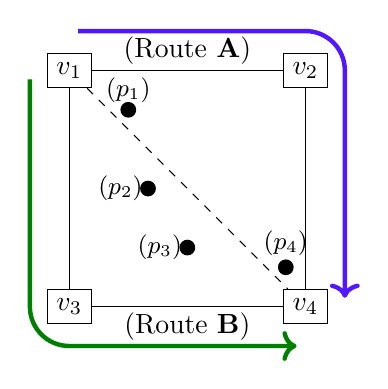
\begin{tikzpicture} 
%[every node/.style={circle,fill=white}] 
%\node (text1) at (-4,3.2) {\hspace{-52.5mm}\bu $V=\{v_1,v_2,v_3,v_4\}$,};
%\node (text2) at (-4,2.7) {\hspace{-35mm}$E=\{v_1v_2,v_2v_4,v_1v_3,v_3v_4\}$.};
%\node (text3) at (1.8,4.2) {\hspace{-8.3mm}\bu $\mathbf{p}=\{p_{1},p_{2},p_{3},p_{4}\}$};
%(-6.0,2.0)
%\node (text4) at (-4,1.0) {\hspace{-45.1mm}\bu \hanpurple(Route) $\hanpurple(\mathbf{A})=\{v_1v_2,v_2v_4\}$.};
%\node (text5) at (-4,0.5) {\hspace{-44.7mm}\bu \officegreen(Route) $\officegreen(\mathbf{B})=\{v_1v_3,v_3v_4\}$.};
\node (p1) at (0.75,2.75) {{\small \red($p_{1}$)}};
\node (p2) at (0.65,1.5) {{\small \red($p_{2}$)}};
\node (p3) at (1.15,0.75) {{\small \red($p_{3}$)}};
\node (p4) at (2.75,0.8) {{\small \red($p_{4}$)}};
\draw (0,3) node (v1) [draw] {$v_1$};
\draw (3,3) node (v2) [draw] {$v_2$};
\draw (0,0) node (v3) [draw] {$v_3$};
\draw (3,0) node (v4) [draw] {$v_4$};
\draw (v1)--(v2);
\draw (v2)--(v4);
\draw (v4)--(v3);
\draw (v3)--(v1);
\draw[dashed] (v1)--(v4);
%\draw[red, dashed] (p3)--(pn-1);
%\draw[red, dashed] (p2)--(pn);
\node at (1.5,3.25) {{\hanpurple(Route $\mathbf{A}$)}};
\node at (1.5,-0.25) {{\green(Route $\mathbf{B}$)}};
\path[arrows=->, ultra thick, draw=hanpurple] ($(v1)+(0.1125,0.5)$) 
to[out=0,in=180] ($(v2)+(0,0.5)$)
to[out=0,in=90] ($(v2)+(0.5,0)$)
to[out=270,in=90] ($(v4)+(0.5,0.1125)$);
\path[arrows=->, ultra thick, draw=officegreen] ($(v1)+(-0.5,-0.1125)$) 
to[out=270,in=90] ($(v3)+(-0.5,0)$)
to[out=270,in=180] ($(v3)+(0,-0.5)$)
to[out=0,in=180] ($(v4)+(-0.1125,-0.5)$);
\fill (0.75,2.5) circle(0.1);
\fill (1,1.5) circle(0.1);
\fill (1.5,0.75) circle(0.1);
\fill (2.75,0.5) circle(0.1);
\end{tikzpicture}
\end{center}
\end{minipage}
%%%%%%%%%%%%%%%%%%%%%%%%%%%%
\begin{minipage}{0.1\hsize}
\begin{center}
\end{center}
\end{minipage}
%%%%%%%%%%%%%%%%%%%%%%%%%%%%
\begin{minipage}{0.43\hsize}
\begin{center}
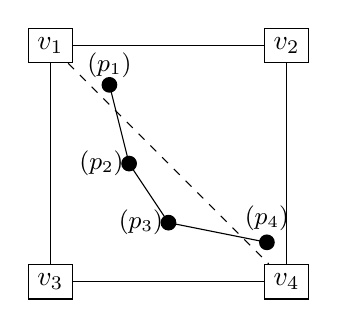
\begin{tikzpicture}%[every node/.style={circle,fill=white}]
\node (p1) at (0.75,2.75) {{\small \red($p_{1}$)}};
\node (p2) at (0.65,1.5) {{\small \red($p_{2}$)}};
\node (p3) at (1.15,0.75) {{\small \red($p_{3}$)}};
\node (p4) at (2.75,0.8) {{\small \red($p_{4}$)}};
\draw (0,3) node (v1) [draw] {$v_1$};
\draw (3,3) node (v2) [draw] {$v_2$};
\draw (0,0) node (v3) [draw] {$v_3$};
\draw (3,0) node (v4) [draw] {$v_4$};
\draw (v1)--(v2);
\draw (v2)--(v4);
\draw (v4)--(v3);
\draw (v3)--(v1);
\draw[dashed] (v1)--(v4);
\draw (0.75,2.5)--(1,1.5);
\draw (1,1.5)--(1.5,0.75);
\draw (1.5,0.75)--(2.75,0.5);
%\draw[red, dashed] (p3)--(pn-1);
%\draw[red, dashed] (p2)--(pn);
%\node at (1.5,3.25) {{\hanpurple(Route $\mathbf{A}$)}};
%\node at (1.5,-0.25) {{\officegreen(Route $\mathbf{B}$)}};
%\path[arrows=->, ultra thick, draw=hanpurple] ($(v1)+(0.1125,0.5)$) 
%to[out=0,in=180] ($(v2)+(0,0.5)$)
%to[out=0,in=90] ($(v2)+(0.5,0)$)
%to[out=270,in=90] ($(v4)+(0.5,0.1125)$);
%\path[arrows=->, ultra thick, draw=officegreen] ($(v1)+(-0.5,-0.1125)$) 
%to[out=270,in=90] ($(v3)+(-0.5,0)$)
%to[out=270,in=180] ($(v3)+(0,-0.5)$)
%to[out=0,in=180] ($(v4)+(-0.1125,-0.5)$);
\fill (0.75,2.5) circle(0.1);
\fill (1,1.5) circle(0.1);
\fill (1.5,0.75) circle(0.1);
\fill (2.75,0.5) circle(0.1);
\end{tikzpicture}
%\vspace{-4mm}
\caption{{\footnotesize Connecting trajectory points.}} 
\end{center}
\end{minipage}
\end{tabular}
\end{figure}
\begin{tcolorbox}[colframe=yellow,
colback=yellow!10!white,
colbacktitle=yellow!40!white,
coltitle=black, fonttitle=\bfseries]
\begin{itemize}
    \item
    Considering not only trajectory points, but also the entire polyline.  
    \item
    Comparing it with the entirety of each route. %(``trajectory segments-to-route'')
\end{itemize}
%\textbf{Aim}: Comparing two entire routes rather than each edges. 
\end{tcolorbox}
%\hrulefill
\end{frame}

\begin{frame}{``Electrical charge'' method}
\begin{enumerate}
    \item
    Giving the candidate routes and polyline opposing electrical charges. 
    \item
    Choosing the route which exerts the most force on the polyline as the true route.
\end{enumerate}
\vspace{-4mm}
\begin{figure}[H]
\begin{tabular}{ccc}
\begin{minipage}{0.43\hsize}
\begin{center}
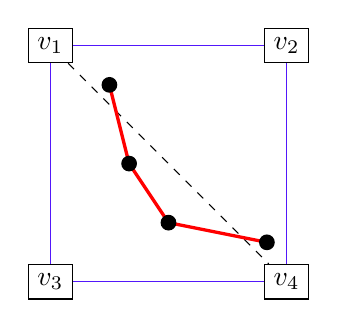
\begin{tikzpicture}%[every node/.style={circle,fill=white}]
\draw (0,3) node (v1) [draw] {$v_1$};
\draw (3,3) node (v2) [draw] {$v_2$};
\draw (0,0) node (v3) [draw] {$v_3$};
\draw (3,0) node (v4) [draw] {$v_4$};
%\node (x) at (1.5,3) {};
%\node (y) at (1.5,-0.5) {};
\draw[hanpurple] (v1)--(v2);
\draw[hanpurple] (v2)--(v4);
\draw[hanpurple] (v4)--(v3);
\draw[hanpurple] (v3)--(v1);
\draw[dashed] (v1)--(v4);
\draw[red, very thick] (0.75,2.5)--(1,1.5);
\draw[red, very thick] (1,1.5)--(1.5,0.75);
\draw[red, very thick] (1.5,0.75)--(2.75,0.5);
\fill (0.75,2.5) circle(0.1);
\fill (1,1.5) circle(0.1);
\fill (1.5,0.75) circle(0.1);
\fill (2.75,0.5) circle(0.1);
%\draw[red, dashed] (p1)--(pn-1);
%\draw[red, dashed] (p2)--(pn);
\end{tikzpicture}
%\vspace{-4mm}
\caption{{\footnotesize Giving electrical charges.}}
\end{center}
\end{minipage}
%%%%%%%%%%%%%%%%%%%%%%%%%%%%
\begin{minipage}{0.1\hsize}
\begin{center}
\end{center}
\end{minipage}
%%%%%%%%%%%%%%%%%%%%%%%%%%%%
\begin{minipage}{0.43\hsize}
\begin{center}
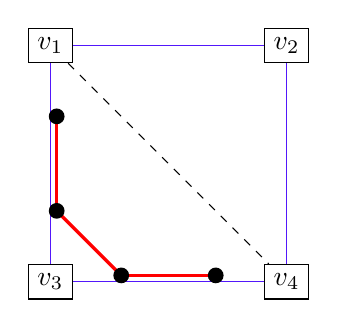
\begin{tikzpicture}%[every node/.style={circle,fill=white}]
\draw (0,3) node (v1) [draw] {$v_1$};
\draw (3,3) node (v2) [draw] {$v_2$};
\draw (0,0) node (v3) [draw] {$v_3$};
\draw (3,0) node (v4) [draw] {$v_4$};
\draw[hanpurple] (v1)--(v2);
\draw[hanpurple] (v2)--(v4);
\draw[hanpurple] (v4)--(v3);
\draw[hanpurple] (v3)--(v1);
\draw[dashed] (v1)--(v4);
\draw[red, very thick] (0.08,2.1)--(0.08,0.9);
\draw[red, very thick] (0.08,0.9)--(0.9,0.08);
\draw[red, very thick] (0.9,0.08)--(2.1,0.08);
\fill (0.08,2.1) circle(0.1);
\fill (0.08,0.9) circle(0.1);
\fill (0.9,0.08) circle(0.1);
\fill (2.1,0.08) circle(0.1);
\end{tikzpicture}
%\vspace{-4mm}
\caption{{\footnotesize Moving to ``closer'' route.}} 
\end{center}
\end{minipage}
\end{tabular}
\end{figure} 
%\hrulefill
\end{frame}


\begin{frame}{``Electrical charge'' method}
\begin{tcolorbox}[colframe=yellow,
colback=yellow!10!white,
colbacktitle=yellow!40!white,
coltitle=black, fonttitle=\bfseries]
\textbf{Further problem}: 
Taking into account information such as
\begin{itemize}
    \item
    speed,
    \item
    direction,
    \item
    error.
\end{itemize}
\end{tcolorbox}

\begin{itemize}
    \item
    Varying the electric density instead of assuming uniformity.
\end{itemize}
\end{frame}


%%%%%%%%%%%%%%%%%%%%%%%%%%%%%%%%%%%%%%%%%%%%%%%%%%%%%
%%%%%%%%%%%%%%%%%%%%%%%%%%%%%%%%%%%%%%%%%%%%%%%%%%%%%
\section{Implementation}
\begin{frame}{Jupyter Demonstration}
\centering
\includegraphics[height=0.7\paperheight,keepaspectratio]{Jupyter Notebook LaTeX/output_3_0.png}

\end{frame}

\begin{frame}{Datasets}
    
After formulating the proposed  mathematical methods into robust map-matching algorithms, we will implement them in python to evaluate their performance numerically using these datasets:
\begin{itemize}
    \item \textit{Dataset for testing and training of map-matching algorithms} \cite{KCMMN} (GPS only, has ground truths),
    \item The BDD100K open data set provided by Berkeley \cite{yuBDD100KDiverseDriving2020} (for GPS and IMU data, no ground truths).\footnote{Because there are no public annotated ground truths, we compare our predictions with the standard EKF approach. This evaluation method is flawed but unavoidable.} % Describe what we used for ground truths
\end{itemize}
We will also compare the performance of our methods to a geometric method, such as point-to-curve, and HMM method, such as an extended Kalman filter (EKF) or Fast Map-Matching \cite{YG}.
    
\end{frame}

\begin{frame}{Evaluation}
    How do we measure the accuracy of our prediction? 
    
    \vspace{-2.5mm}
    \begin{figure}[ht]
    \centering
    \def\svgwidth{\linewidth}
    {\footnotesize
    \input{error-formula.pdf_tex}}
    \footnotesize
    \begin{align*} 
	    d_0 &= \text{length of ground truth} \\
	    d_- &= \text{length of prediction route erroneously subtracted} \\
	    d_{+} &= \text{length of prediction route erroneously added}
    \end{align*}
    \normalsize
    \caption{Error Formula by Newson and Krumm}
    \label{fig:error-formula}
\end{figure}
    
\end{frame}

\begin{frame}
\frametitle{Thank You! And References}

\begin{thebibliography}{9}
\scriptsize{
% \bibitem{KB} Kolmogorov, A. N. and Barzdin, Ya. M.; On the realization of networks in three-dimensional space, in
% \textit{Selected Works of Kolmogorov}, Volume 3, ed. Shiryaev, A. N., Kluwer Academic Publishers, Dordrecht,
% 1993.


\bibitem[H]{H}  High-assurance Mobility Control Lab. \url{https://hmc.unist.ac.kr/research/autonomous-driving/}
\bibitem[KCMMN]{KCMMN} M. Kubi\u cka, A. Cela, P. Moulin, H. Mountier and S. I. Niculescu, \textit{Dataset for testing and training of map-matching algorithms}, In 2015 IEEE Intelligent Vehicles Symposium (IV), 1088--1093 (2015).
\bibitem[Sa]{Sa} F. Santambrogio, \textit{Optimal transport for applied mathematicians. Calculus of variations, PDEs, and modeling}, Progress in Nonlinear Differential Equations and their Applications, Birkh\"{a}user/Springer, Cham. (2015).
\bibitem[YCWXCLMD]{yuBDD100KDiverseDriving2020} F. Yu, H. Chen, X. Wang, W. Xian, Y. Chen, F. Liu, V. Madhavan and T. Darrell, \textit{BDD100K: A Diverse Driving Dataset for Heterogeneous Multitask Learning}, In Proceedings of the IEEE/CVF conference on computer vision and pattern recognition, 2636--2645 (2020).
\bibitem[YG]{YG} C. Yang and G. Gid\' ofalvi, \textit{Fast map matching, an algorithm for integrating a hidden Markov model with precomputation}, International Journal of Geographical Information Science. Taylor \& Francis, \textbf{32}(3), 547--570 (2018).}
\end{thebibliography}

\end{frame}

\end{document}